\ifdefined\XeTeXversion
\else
  \pdfoutput=1
\fi
\documentclass[11pt]{article}

\usepackage{axym-publication}
\usepackage[utf8]{inputenc}
\usepackage[T1]{fontenc}
\usepackage{microtype}
\usepackage{amsmath,amssymb,amsfonts,mathtools}
\usepackage{graphicx}
\usepackage{booktabs}
\usepackage{float}
\usepackage{nicefrac}
\usepackage[numbers,sort&compress]{natbib}
\usepackage{hyperref}
\usepackage{cleveref}
\usepackage{url}
\usepackage{doi}

\publicationtitle{Improved Elastic Weight Consolidation as an Optimization Constraint for Continual Learning}
\publicationauthors{Davide Wiest}
\publicationaffiliations{Department of Computer Science, TU Darmstadt; Independent Researcher\\Darmstadt, Germany}
\publicationdate{2026}
\publicationcode{https://github.com/Axym-Labs/iewc}
\publicationprojectpage{https://axym.org/work/iewc}
\publicationcorrespondence{dw@axym.org}

\hypersetup{
  pdftitle={Improved Elastic Weight Consolidation as an Optimization Constraint for Continual Learning},
  pdfauthor={Davide Wiest},
  pdfkeywords={continual learning, elastic weight consolidation, empirical Fisher, constrained optimization},
}

\begin{document}
\makepublicationtitle

\publicationleadfigure[0.36\textheight]{figures/overview.pdf}{%
Each surface shows the continual-learning penalty over normalized directions,
which locally approximate loss changes for two representative samples.
Observed-label OPG/EWC induces anisotropy through gradient-scale weighting;
uniform IEWC removes this scaling away from the damping regime, while the
separate RDW variant weights samples by streaming residual diversity.
\citep{GSS}}

\publicationabstract{Elastic Weight Consolidation (EWC) is widely used in continual learning, and standard implementations use the empirical Fisher matrix, whose justification beyond probabilistic classification remains incomplete. The empirical Fisher differs from the true Fisher, aligns with it only under specific assumptions, and is nevertheless used broadly in practice. We address this gap by deriving EWC from first principles. Starting from the continual-learning problem, we formulate old-task solution preservation as a constrained optimization problem (CLOC) and develop PL-CLOC, a population, low-order variant for deriving scalable mechanisms. Within this framework, preserving the old scalar loss value recovers exactly the empirical Fisher matrix (EF) used in EWC. This places empirical-Fisher EWC on direct optimization-theoretic footing without reliance on the true Fisher matrix. Preserving outputs up to motion along the old-task loss level set recovers the improved empirical Fisher (IEF) and leads to IEWC, a generalized and normalized sibling of EWC. EF implicitly scales local old-task sensitivity directions by the output's gradient magnitude, whereas IEF does not. We identify EWC-DR's vanishing-importance pathology as a special case of this gradient-scale effect on well-fitted data, and provide the improved empirical Fisher as the general solution. More broadly, the derivation separates the outer EWC mechanism from output geometry, enabling geometry-aware continual learning within the same regularization template. Empirically, across image classification, continual LLM/NLP, segmentation, forecasting, and diffusion, IEWC improves final average performance in two settings and, with sample weighting, improves performance across all tested settings. Together, these results motivate IEWC as a theoretical and practical successor.}

\makepublicationlinks
\clearpage

\section{Continual Learning as Optimization Constraint}

Consider the problem of continual learning, where data from distributions (tasks, environments) are presented sequentially \citep{McCloskeyCohen1989,French1999,Parisi2019,VanDeVenTolias2019}. Concretely, we first train a model on distribution $A$ and obtain parameters $\theta^*_A$, and only then can we optimize with respect to a new distribution $B$. If we plainly pick a minimal loss/cost $\min_\theta L_B(\theta)$ as our objective, then the optimization does not have to respect performance on $A$, which usually degrades it too much to be practical. Hence, we have to guide or constrain optimization in a way. A natural fit for this problem is the framework of constrained optimization, with solution preservation being the constraint in question. Define both a quantity $Q: \Theta \rightarrow \mathcal{H}$ that is relevant to this preservation and a constraint set $\mathcal{C} \subset \mathcal{H}$ that implies preservation is met. Before exploring concrete choices in later sections, we continue on the common thread. These two objects let us define a new objective:
\[
\min_{\theta \in \Theta} L_B(\theta)
\qquad
\text{subject to}
\qquad
q(\theta) \in \mathcal{C}
\]
This gives a mathematical formulation of preservation, and the next section extends it to become more practical.


\section{Related Work and Scope}
\label{sec:related-work}

EWC stores a quadratic approximation around earlier parameters and weights parameter motion by a Fisher-derived importance estimate \citep{EWC}. Other parameter-importance regularizers estimate importance from the optimization trajectory, output sensitivity, or a combination of EWC-style curvature and path-integral evidence \citep{SI,MAS,RWalk}; their apparently different estimators have also been analyzed within a common framework \citep{BenzingRegularisation}. Bayesian and posterior-combination approaches instead accumulate task posteriors or merge their moments \citep{ProgressCompress,VCL,IMM}. A practical ambiguity remains: implementations called ``Fisher'' may use the model-label expectation, sampled model labels, observed labels, or minibatch aggregates. These estimators are not interchangeable in theory or practice \citep{KunstnerEF,VanDeVenFisher2025}. Our scalar-loss derivation concerns the observed-label OPG object; sampled model-Fisher EWC is evaluated separately rather than treated as another name for the same matrix.

Regularization can instead protect functions or representations. LwF distills old predictions on later inputs, encoder-based lifelong learning constrains reconstructions of old-task features, and functional regularization preserves selected predictive functions or memorable points \citep{LwF,EBLL,FunctionalGP,FROMP}. More generally, many training objectives contain vectors or matrices that are computed from parameters or activations but held constant with respect to the parameters being optimized, such as weight-averaged teacher parameters \citep{MeanTeacher}, stop-gradient target projections \citep{BYOL,SimSiam}, predictions of an earlier model \citep{LwF}, and running activation moments \citep{TeReL}. EWC and IEWC follow the same pattern in the sense that both compute an importance matrix once earlier tasks are learned and then hold it fixed as the weighting of a quadratic penalty. CLOC complements this taxonomy: it begins with a preservation specification and asks which local stored penalty follows. The algebra below allows differentiable scalar functionals, while IEWC specializes to scalar-loss preservation and loss-level-set-normal output preservation.

iEF was introduced as a normalized observed-gradient approximation for natural-gradient optimization \citep{IEF}. We recover its Euclidean algebra from a different question: the metric distance of an old output displacement from the tangent to its old loss level set. This provides a preservation interpretation but does not convert iEF into exact global curvature. Our additions relative to simply substituting iEF into EWC are the CLOC derivation, the matched output-metric generalization, the finite-damping and interpolation boundary, and the separation of normalization from aggregation weights. The RDW ablation borrows a streaming residual-diversity intuition from GSS \citep{GSS}; it is an explicitly order-dependent heuristic, not part of the level-set result.


\section{Population and Local Approximations}

To obtain a differentiable objective suitable for gradient-based optimization, we apply the standard Moreau-Yosida regularization of the constraint indicator, which for closed convex $\mathcal C$ yields the squared-distance penalty \citep{MoreauProx}:
\[
\min_\theta J(\theta)=
\min_\theta L_B(\theta) + \frac{\lambda}{2}\text{dist}(q(\theta), \mathcal{C})^2 = 
\min_\theta L_B(\theta) + \frac{\lambda}{2}\inf_{u \in \mathcal{C}} \ \text{dist}(q(\theta), u)^2.
\]
We call this the \textbf{Continual Learning as Optimization Constraint (CLOC)} formulation. GEM and A-GEM are similar in spirit in that they formulate preservation through constraints on old examples \citep{GEM,AGEM}. CLOC turns the old-task constraint into a proximal penalty built after task-$A$ training. In a population setting, e.g. when we have a dataset, we can translate this into a population risk objective by wrapping it in an expectation over the data and using sample-based analogues $\ell_B$ of $L_B$ and $q$ of $Q$, then taking the empirical average. Define the unscaled proximal loss as $p(a, \theta)=\text{dist}(q(a, \theta), \mathcal{C})^2$.
\[
\min_\theta
\;
\frac{1}{N_B}\sum_{i=1}^{N_B}\ell_B(b_i,\theta)
+
\frac{\lambda}{2N_A}\sum_{i=1}^{N_A}p(a_i, \theta)
\]
The two-distribution presentation is only for notational simplicity; additional old distributions can be handled by adding analogous constraints. We refer to this population version as \textbf{population CLOC (P-CLOC)}. One efficiency consideration is the penalty $p$: Ideally, we let the constraint contribute to each gradient step with its gradient. However, recomputing the full old-distribution penalty $p$ and its associated factors many times during optimization on distribution $B$ is usually prohibitively expensive, since it depends on the dataset $D_A$ associated with $A$. Additionally, reusing dataset $D_A$ later on does not respect the continual learning setting. For this reason, replace the exact penalty by a local $k$-th order Taylor-polynomial approximation around the old solution $\theta_A^\star$.
This turns the computation of $p$ into a repeated evaluation of precomputed derivative tensors and bounds memory requirements to $O(d^k)$ for a $d$-dimensional parameterization. Since memory scales exponentially with $k$, the standard scalable surrogate is a low-order Taylor approximation. We refer to this local approximation as \textbf{low-order CLOC (L-CLOC)}, and to its population version as \textbf{PL-CLOC}. It remains to specify the preserved quantity $q$ and constraint set $\mathcal{C}$. Notice that the gradient of $p$ is dependent on only one sample at once, which allows us to analyze $p$ and its gradients on a per-sample basis.


\section{Old-Task Loss Preservation}

Since $\ell_A$ is our best practical surrogate on performance on distribution $A$, a natural choice is to use $\ell_A$ itself to define preservation. We say that the model $f_\theta$ preserved the solution if it preserved the old loss value for distribution $A$. This leads to:
\[
q(a,\theta)
=
\ell_A(f_\theta(x))-\ell_A(f_{\theta_A^\star}(x)).
\]
Since preservation means $q(a,\theta)=0$, take $\mathcal C=\{0\}$. The corresponding unscaled proximal loss is
\[
p(a,\theta)
=
\operatorname{dist}(q(a,\theta),\mathcal C)^2
=
q(a,\theta)^2.
\]
To obtain a low-order Taylor approximation, use the perturbation around the old solution $\delta=\theta-\theta_A^\star$ in the first-order expansion of $q$:
\[
q(a,\theta_A^\star+\delta)
\approx
g^\top\delta,
\]
where
\[
g
=
\nabla_\theta \ell_A(f_{\theta_A^\star}(a)).
\]

Equivalently, writing
\[
z_A=f_{\theta_A^\star}(a)
\qquad
r_i
=
\nabla_z \ell_A(z)\big|_{z=f_{\theta_A^\star}(a)},
\qquad
J_i
=
\nabla_\theta f_{\theta_A^\star}(a),
\]
the chain rule gives
\[
g_i
=
J_i^\top r_i.
\]

Substituting this expansion into the preservation penalty gives
\[
\frac{\lambda}{2N_A}\sum_{i=1}^{N_A} q(a_i,\theta)^2
\;\approx\;
\frac{\lambda}{2N_A}\sum_{i=1}^{N_A} (g_i^\top\delta)^2.
\]
Collecting the gradient outer products yields
\[
\frac{\lambda}{2N_A}\sum_{i=1}^{N_A} (g_i^\top\delta)^2
=
\frac{\lambda}{2}\,
\delta^\top
\left(
\frac{1}{N_A}\sum_{i=1}^{N_A} g_i g_i^\top
\right)
\delta
=
\frac{\lambda}{2}\,
\delta^\top
M_1
\delta.
\]

Therefore the resulting matrix is
\[
M_1
=
\frac{1}{N_A}\sum_{i=1}^{N_A} g_i g_i^\top
=
\frac{1}{N_A}\sum_{i=1}^{N_A} J_i^\top r_i r_i^\top J_i.
\]
We call this an importance matrix as it encodes how important it is to preserve a direction in parameter space.


\section{Empirical Fisher Regularization}

This is exactly the empirical Fisher matrix $F_{\mathrm{EF}}$, the standard practical matrix used in Elastic Weight Consolidation (EWC) \citep{EWC}. We refer to this instantiation as EF-EWC:
\[
M_1=F_{\mathrm{EF}}.
\]
Hence EF-EWC approximates a constrained optimization problem with a smooth proximal penalty, preserving the old scalar loss value sample by sample. This places EF-EWC within the broader family of parameter-importance regularizers \citep{SI,MAS} and Bayesian or online continual-learning approximations \citep{HuszarEWC,ProgressCompress,VCL}.

The original EF-EWC derivation uses properties specific to probabilistic classification models. After training on task $A$, one considers the posterior over parameters
\[
p(\theta\mid \mathcal D_A)\propto p(\mathcal D_A\mid \theta)\,p(\theta),
\]
and uses it as a prior when learning task $B$. Expanding the negative log-posterior around the old solution $\theta_A^\star$ yields a local quadratic approximation
\[
-\log p(\theta\mid \mathcal D_A)
\approx
-\log p(\theta_A^\star\mid \mathcal D_A)
+
\frac12(\theta-\theta_A^\star)^\top H_A(\theta_A^\star)(\theta-\theta_A^\star),
\]
where $H_A(\theta_A^\star)$ is the Hessian of the negative log-posterior at the old solution. Under the usual assumptions for log-likelihood models, and neglecting the prior curvature term or absorbing it into the approximation, this Hessian can be replaced by the Fisher information matrix
\[
F(\theta)
=
\mathbb E_{(x,y)\sim\mathcal D_A}
\left[
\nabla_\theta \log p_\theta(y\mid x)\,
\nabla_\theta \log p_\theta(y\mid x)^\top
\right].
\]

For negative log-likelihood losses, this Fisher matrix coincides with the curvature of the expected loss under standard regularity conditions, and therefore matches the corresponding Hessian-based local quadratic model near an optimum, as in the natural-gradient and approximate-curvature literature \citep{Amari1998,MartensNG,KFAC}. Since classification models explicitly define a predictive distribution $p_\theta(y\mid x)$ over labels, the true Fisher can be computed as population object by sampling from said distribution. In practice, however, EWC replaces it by empirical approximations computed from the old dataset, which leads to the empirical Fisher form used above. However, this framework leaves open a justification of the empirical Fisher outside of negative log-likelihood losses. This is an open problem because EWC is used for different tasks and objectives as well, for example for diffusion \citep{Rank1Diffusion}. Furthermore, Kunstner et al. show that the empirical Fisher is a different mathematical object than the true Fisher and approximates the true Fisher well only in specific settings \citep{KunstnerEF}. We re-derive EF-EWC from scratch using PL-CLOC to resolve these two issues, basing the usage of said matrix on solid theoretical grounding without reliance on the true Fisher matrix.


\section{Level-Set Preservation in Output Space}

Section~\ref{sec:scalar-functional-preservation} preserves a scalar functional value directly. A second construction instead preserves the model output up to motions along a level set of a differentiable output functional $\phi_a:\mathcal Z\to\mathbb R$. This output-space perspective connects to distillation and functional regularization approaches to continual learning \citep{LwF,Distillation,FunctionalGP,FROMP}. Let $a \in D_A$ be an old sample, write $z_A=f_{\theta_A^\star}(x)$, and define the exact preservation set
\[
\mathcal C_a=
\{z:\phi_a(z)=\phi_a(z_A)\}.
\]
Thus the preserved quantity is the model output itself:
\[
q(a,\theta)=f_\theta(x).  
\]
The hard constraint is
\[
q(a,\theta)\in\mathcal C_a,
\]
and the corresponding unscaled proximal loss is
\[
p(a,\theta) =
\operatorname{dist}_{G}\big(q(a,\theta),\mathcal C_a\big)^2,
\]
where $G\succ0$ is the chosen local output metric. Positive definiteness makes the primal metric and its inverse on covectors unambiguous; Section~\ref{sec:output-geometry} treats the restricted pseudoinverse convention needed by a singular ordered-output example.

We obtain a tractable penalty from the standard first-order model of the constraint set near $z_A$, namely its tangent plane. Let
\[
r=
\nabla_z \phi_a(z)\big|_{z=z_A}.
\]
We first assume $r\ne0$, so the functional's level set has a regular tangent hyperplane at $z_A$.
For a small output displacement $\Delta z=f_\theta(x)-f_{\theta_A^\star}(x)$, its first-order change is approximately $r^\top \Delta z$.
Hence the local constraint set is
\[
T=
\{\Delta z:r^\top \Delta z=0\}.  
\]
Replacing the exact level set by this tangent hyperplane gives the local proximal loss
\[
p(a,\theta)  
\approx  
\operatorname{dist}_{G}(\Delta z,T)^2.  
\]

For the metric $|v|_G^2=v^\top G v$, the squared distance to the tangent hyperplane follows from projecting $\Delta z$ onto the gradient:
\[
\operatorname{dist}_{G}(\Delta z,T)^2 =
\frac{(r^\top \Delta z)^2}{r^\top G^{-1}r}.  
\]
To verify the matched metric pair, write the normal residual as $e=\Delta z-t$ with $t\in T$. It solves
\[
\min_e e^\top G e
\quad\text{subject to}\quad
r^\top e=r^\top\Delta z.
\]
The Lagrange equations give
\[
e^\star
=
\frac{r^\top\Delta z}{r^\top G^{-1}r}G^{-1}r,
\]
whose squared $G$-norm is the displayed quotient. Thus $G$ measures primal output displacement while $G^{-1}$ acts on the loss covector; these roles cannot be chosen independently.
Linearizing the model output around $\theta_A^\star$, with
\[
\delta=\theta-\theta_A^\star,  
\qquad  
J=\nabla_\theta f_{\theta_A^\star}(x),  
\]
we have
\[
\Delta z \approx J\delta.  
\]
Substituting this into the local regularization term gives
\[
\frac{\lambda}{2}p(a,\theta_A^\star+\delta)  
\approx  
\frac{\lambda}{2}  
\frac{(r^\top J\delta)^2}{r^\top G^{-1}r}.  
\]
Equivalently,
\[
\frac{\lambda}{2}p(a,\theta_A^\star+\delta)  
\approx  
\frac{\lambda}{2}  
\delta^\top  
\left(
J^\top  
\frac{rr^\top}{r^\top G^{-1}r}  
J  
\right)
\delta.  
\]

Taking the empirical average over old-distribution samples $a_1,\dots,a_N$ yields an importance matrix of the form
\[
M_{2,A} =
\frac{1}{N}\sum_{i=1}^N  
J_i^\top  
\frac{r_i r_i^\top}{r_i^\top G_i^{-1}r_i}  
J_i.  
\]

This local construction penalizes motion normal to the tangent model. IEWC is the evaluated specialization $\phi_a=\ell_A$; other functionals define CLOC extensions. When $r_i=0$, the tangent normal is undefined and the undamped quotient is $0/0$; our finite-damping implementation assigns that sample zero contribution. Section~\ref{sec:well-fitted} characterizes the resulting near-interpolation behavior.


\subsection{Level-Set Normalization and the Improved Empirical Fisher}

For the loss-functional specialization $\phi_a=\ell_A$ and Euclidean output metric $G_i=I$, the matrix from the previous section is the improved empirical Fisher (iEF) introduced by Wu et al. \citep{IEF}:
\[
M_{2,I}=F_{\mathrm{IEF}}.
\]
Hence iEF is the quadratic form of a first-order local constraint that protects old behavior geometrically: instead of preserving a raw scalar-loss coordinate, it penalizes only output motion normal to the old loss level set. The original iEF paper derives the same normalization for approximate natural-gradient descent. In that setting, the observed-label OPG reweights sample contributions by squared output-gradient magnitude; iEF removes this scale factor and retains the normalized output-loss direction. Here the normalization arises from metric projection onto the normal quotient of the old-loss tangent space.

Consider the scalar least-squares setting in Euclidean geometry. Suppose the model output is scalar, such that
\[
\ell_n(z)=\frac12(z-y_n)^2.
\]
Then
\[
r_n=z_n^A-y_n
\]
is scalar, and for $r_n\neq 0$ we have
\[
\frac{r_n^2}{r_n^2}=1.
\]
Therefore the \emph{undamped} Euclidean IEF contribution reduces to
\[
J_n^\top J_n,
\]
and averaging gives
\[
M_{\mathrm{IEF}}
=
\frac{1}{N}\sum_{n=1}^N J_n^\top J_n.
\]
This is exactly the Gauss--Newton or output-Jacobian form for squared-error regression \citep{GaussNewton,MartensHF,MartensNG}, the standard practical preconditioning matrix for second-order optimization. This matches our geometric intuition: loss preservation is governed by how parameters move the output, which is encoded by the Jacobian $J$, not by the current output-gradient magnitude. This equivalence was made explicit in \citep{IEF}.


\section{Relation to Gauss-Newton}

Consider the scalar least-squares setting in Euclidean geometry. Suppose the model output is scalar, such that
\[
\ell_n(z)=\frac12(z-y_n)^2.
\]
Then
\[
r_n=z_n^A-y_n
\]
is scalar, and for $r_n\neq 0$ we have
\[
\frac{r_n^2}{r_n^2}=1.
\]
Therefore the Euclidean IEF contribution reduces to
\[
J_n^\top J_n,
\]
and averaging gives
\[
M_{\mathrm{IEF}}
=
\frac{1}{N}\sum_{n=1}^N J_n^\top J_n.
\]
This is exactly the Gauss--Newton or output-Jacobian form for squared-error regression \citep{GaussNewton,MartensHF,MartensNG}, the standard practical preconditioning matrix for second-order optimization. This matches our geometric intuition: Loss preservation is governed by how parameters move the output, which is encoded by the Jacobian $J$, not by the current output gradient magnitude. This equivalence was made explicit in \citep{IEF}. In fact, the IEF was motivated as an approximate Gauss--Newton algorithm.


\section{Normalization and Sample Weighting}

To compare both matrices in a common notation, let $G_n\succ0$ denote the chosen output metric for sample $n$. Although $M_{\mathrm{OPG}}$ itself does not depend on $G_n$, its summands can be rewritten relative to that metric. In a negative-log-likelihood setting, $M_{\mathrm{OPG}}=F_{\mathrm{emp}}$.

Define
\[
\hat r_n^{\,G}
=
\frac{r_n}{\sqrt{r_n^\top G_n^{-1}r_n}},
\qquad
a_n^{\,G}
=
J_n^\top \hat r_n^{\,G},
\qquad
w_n^{\,G}
=
r_n^\top G_n^{-1}r_n.
\]
Then, wherever $r_n\ne0$,
\[
M_{\mathrm{IEF},G}
=
\frac{1}{N}\sum_{n=1}^N a_n^{\,G}(a_n^{\,G})^\top,
\qquad
M_{\mathrm{OPG}}
=
\frac{1}{N}\sum_{n=1}^N w_n^{\,G}\,a_n^{\,G}(a_n^{\,G})^\top.
\]

If we interpret both matrices as empirical aggregates of local old-task sensitivity directions $a_n^{\,G}(a_n^{\,G})^\top$, they use the same directions but differ in how strongly each sample contributes. Undamped IEF keeps uniform empirical weighting of these normalized directions, while OPG multiplies each contribution by the metric-dependent squared magnitude
\[
w_n^{\,G}=r_n^\top G_n^{-1}r_n.
\]

Thus normalization changes sample aggregation: OPG shifts old-task weighting toward samples with large output-loss gradients and away from confidently fitted ones, whereas undamped IEF removes that scale. With positive damping, IEF also multiplies each direction by $s_n/(s_n+\tau)$, as Section~10 makes explicit.

This decomposition identifies a mechanism to test; it does not show that either weighting is preferable for every task. The next section treats probabilistic classification, where the scale difference has a concrete well-fitted limit.


\section{Gradient-Scale Effects in Classification}

The output-gradient weighting in EF has an important classification-specific symptom. Consider one data sample. For cross-entropy with softmax probabilities $p_n$ and one-hot label $y_n$, the output-loss gradient with respect to logits is
\[
r_n=p_n-y_n.
\]
For a confidently correct prediction with class $c$ and small $\varepsilon$,
\[
p_{n,c}=1-\varepsilon,
\]
we have
\[
\|r_n\|_2^2=\|p_n-y_n\|_2^2 \in \Theta(\varepsilon^2).
\]
Thus the EF contribution of this sample becomes small as the model becomes more confident and correct. This is coherent with the way we derived the EF: the scalar first-order loss change becomes small. In continual learning, this is undesirable: The samples that the old model classifies best may receive very low importance. EWC-DR identifies this failure mode in classification and proposes a classification-specific repair through a logit-reversal operation, literally flipping the signs of the model's logits \citep{EWC-DR}. In the present framework, their observation can be read as a symptom of the weighting issue identified in Section 8: $F_{\mathrm{EF}}$ importance depends on output-gradient scale. This evidently does not occur for $M_{\mathrm{IEF}}$, and we make this point precise in the next section. Hence, the normalization analysis yields a formal problem identification and its generalizable solution, the Improved Empirical Fisher matrix.


\section{Gradient Scale Near Well-Fitted Solutions}
\label{sec:well-fitted}

For softmax cross-entropy with probabilities $p_n$ and one-hot label $y_n$, the output-loss gradient with respect to logits is $r_n=p_n-y_n$. If the correct class has probability $p_{n,c}=1-\varepsilon$, then $\|r_n\|_2^2\in\Theta(\varepsilon^2)$, so the observed-label OPG contribution vanishes quadratically as confidence approaches one. The squared first-order loss change has the same scaling, yet continual-learning importance concerns the cost of changing that prediction later. EWC-DR identifies this classification effect and proposes a logit-reversal repair \citep{EWC-DR}; undamped iEF instead removes the output-gradient scale factor.

The same mechanism extends to arbitrary differentiable losses. Importance is estimated after training on $A$, when many old samples may be well fit. The original EWC Laplace argument likewise expands at an old-task optimum, although its model-Fisher motivation differs from the observed-label OPG analyzed here \citep{EWC,KunstnerEF}. Modern expressive models can fit training data up to interpolation \citep{ModernInterp}, so the near-zero regime must be explicit. For one sample, let
\[
\begin{aligned}
s_n &= r_n^\top G_n^{-1}r_n,\\
S_n^{\mathrm{OPG}} &= J_n^\top r_nr_n^\top J_n,\\
S_{n,\tau}^{\mathrm{IEF},G}
&= \frac{J_n^\top r_nr_n^\top J_n}{s_n+\tau}.
\end{aligned}
\]

\begin{proposition}[Gradient-scale behavior near a well-fitted solution]
\label{prop:well-fitted-scaling}
Assume $m_GI\preceq G_n\preceq M_GI$ and
$\|J_n^\top v\|_2\le C_J\|v\|_2$. For $s_n>0$,
\[
S_n^{\mathrm{OPG}}
=s_nS_{n,0}^{\mathrm{IEF},G},
\qquad
\begin{aligned}
\|S_n^{\mathrm{OPG}}\|_2&\in O(s_n),\\
\|S_{n,0}^{\mathrm{IEF},G}\|_2&\in O(1).
\end{aligned}
\]
If $\|J_n^\top r_n/\sqrt{s_n}\|_2\ge c_J>0$, these rates are
$\Theta(s_n)$ and $\Theta(1)$. Consequently, for Euclidean softmax
cross-entropy with correct-class probability $1-\varepsilon$, they are
$\Theta(\varepsilon^2)$ and $\Theta(1)$, respectively.
\end{proposition}
Appendix~\ref{app:well-fitted-proof} gives the proof.

The proposition isolates the central EWC--IEWC difference. OPG weights each normalized parameter-sensitivity direction by the squared dual norm $s_n$ of the current output-loss gradient; undamped IEF removes that factor while retaining model sensitivity through $J_n$. Current loss-gradient magnitude and the importance of retaining old behavior are therefore distinct quantities.

Positive damping gives $S_{n,\tau}^{\mathrm{IEF},G}=\frac{s_n}{s_n+\tau}S_{n,0}^{\mathrm{IEF},G}$: normalization dominates for $s_n\gg\tau$, whereas $s_n\ll\tau$ suppresses the sample and exact interpolation contributes zero. The confirmatory experiments use $\tau_A=\kappa\operatorname{median}_{s_i>0}s_i$ with $\kappa=10^{-2}$; Appendix~\ref{app:well-fitted-proof} proves invariance to global changes in loss units. If all recorded $s_i$ vanish, the stored importance is zero.


\section{Output-Space Geometry}
\label{sec:output-geometry}

The scalar CLOC construction and its OPG matrix require no output-space metric. The level-set construction does: for a symmetric positive-definite primal metric $G_n$, output displacements have inner product $\langle u,v\rangle_{G_n}=u^\top G_n v$, the metric-normal direction is $G_n^{-1}r_n$, and the normal-distance denominator is $r_n^\top G_n^{-1}r_n$. A valid geometry therefore supplies the matched pair $G_n$ on primal output displacements and $G_n^{-1}$ on loss covectors.

The canonical choice $G_n=I$ recovers iEF \citep{IEF}. More generally, any smooth output discrepancy whose second-order expansion supplies a valid local quadratic metric can enter IEWC through its matched primal/dual pair $G_n,G_n^{-1}$. For singular ambient metrics, this requires a stated tangent space or quotient, Moore--Penrose pseudoinverse, and range conditions; diagonalizing the parameter pullback can further discard cross-parameter geometry.

For ordered probability outputs, Appendix~\ref{app:ordered-cdf-geometry} constructs a CDF/Cram\'er metric and its matched pseudoinverse dual on the simplex tangent. This supplies the space-dependent geometry that motivated the earlier diffusion experiment. That experiment measures the effect of output representation, while the appendix provides the mathematically matched geometric example.


\section{Additional Theoretical Properties}

We move further analysis of $M_{\mathrm{IEF}}$ into the appendix. Namely, we treat invariance to monotone relabelings of the loss and better hyperparameter interpretability in Appendix A, and analyze rank stability of the two matrices subject to a simple contamination model in Appendix B.


\section{Improved Elastic Weight Consolidation}

The preceding derivation leaves five implementation choices: global penalty strength, damping, aggregation weights, output geometry, and matrix approximation. For old-task samples $a_1,\dots,a_N$, IEWC uses
\[
M_{\mathrm{IEWC}}
=
\frac1N
\sum_{n=1}^N
\bar h_n
\frac{g_ng_n^\top}{r_n^\top G_n^{-1}r_n+\tau_A},
\qquad
g_n=J_n^\top r_n,
\]
where $\bar h_n\ge0$ has empirical mean one. The continual-learning penalty is
\[
\frac{\lambda}{2}
(\theta-\theta_A^\star)^\top
M_{\mathrm{IEWC}}
(\theta-\theta_A^\star).
\]

The canonical geometry is $G_n=I$. We use task-relative damping
\[
\tau_A
=
\kappa\,\operatorname{median}
\{r_i^\top G_i^{-1}r_i:r_i\ne0\},
\]
with $\kappa=10^{-2}$ in the confirmatory comparison. This makes $\kappa$ dimensionless and preserves global loss-unit invariance. If all denominators are zero, the stored importance is zero.

Uniform IEWC sets $\bar h_n=1$. To study weighting without confounding it with normalization, we define a separate \emph{residual-diversity weighting} (RDW) variant. Let
\[
u_n=\frac{g_n}{\|g_n\|_2}
\]
for nonzero parameter gradients. In a fixed sample order, RDW maintains an orthonormal basis $Q$ of at most $K$ earlier residual directions and assigns
\[
h_n=\|(I-Q^\top Q)u_n\|_2^2.
\]
When the residual is nonzero and the cap is not reached, its normalized direction is appended to $Q$; the final $h_n$ are mean-normalized. This streaming rule is motivated by residual-gradient diversity ideas in GSS \citep{GSS}, but it is an order-dependent aggregation heuristic, not part of the level-set derivation. Crucially, both OPG-RDW and IEF-RDW receive the same unit parameter-gradient directions. Scalar IEF normalization cannot change $u_n$, so the $2\times2$ comparison
\[
\{\mathrm{OPG},\mathrm{IEF}\}
\times
\{\mathrm{uniform},\mathrm{RDW}\}
\]
isolates matrix normalization from sample weighting.

For diagonal training penalties, we take the diagonal after aggregation and rescale every nonzero diagonal to have mean one over trainable parameters. This removes only a global factor absorbable into $\lambda$ and lets all regularized methods use the same within-domain $\lambda$ grid. It does not restore the cross-parameter information discarded by diagonalization.

An IEWC instantiation is specified by the five-tuple
\[
(\lambda,\kappa,\Gamma,h,\Pi),
\]
where $\lambda$ sets preservation strength, $\kappa$ sets relative damping, $\Gamma$ maps an old output to its local metric $G_n$, $h$ supplies aggregation weights, and $\Pi$ is the matrix approximation operator (for example, full, diagonal, or low rank). These are genuine design choices rather than values fixed by the derivation. Scalar loss preservation gives OPG-EWC; loss-level-set normal preservation gives uniform IEWC. We call this CLOC-derived mechanism \emph{Improved Elastic Weight Consolidation} while treating its individual axes separately in theory and experiment.


\section{Empirical Evaluation}

We next test whether the CLOC-derived regularizers produce useful continual-learning behavior in practical settings. Unless stated otherwise, all EWC matrices are diagonal. We write U-IEWC for the empirical, uniformly weighted IEF aggregation with $h_n\equiv 1$, and GSS-IEWC for a weighted variant that applies the gradient-diversity principle of GSS to the normalized IEWC directions \citep{GSS}. The classification setting is ImageNet-R class-incremental learning with a pretrained ViT-B/16 and LoRA adapters, while the NLP setting is TRACE multiple-choice continual fine-tuning with Qwen2.5-3B and LoRA adapters. Thus, these two setups place the comparison in the recent line of parameter-efficient continual fine-tuning, including LoRA and recent continual LoRA methods \citep{LoRA,FRLoRA,CLLoRA,CLoRA}. We also evaluate non-LoRA fine-tuning of a pretrained CNN for VOC 15-5 semantic segmentation, and from-scratch training for long-horizon time-series forecasting and MNIST DDPM denoising. For each method and task type, we tune $\lambda$ to optimize the average performance metric across distributions; Appendix C gives the full training and tuning protocol, including the selected $\lambda$ and $\tau$ values.

\begin{table}[H]
\centering
\resizebox{\linewidth}{!}{%
\begin{tabular}{llccccc}
\toprule
Task type & Metric & Sequential & EF-EWC & EWC-DR & U-IEWC & GSS-IEWC \\
\midrule
Classification & Final avg. accuracy $\uparrow$ & 0.2896 $\pm$ 0.0405 & 0.5981 $\pm$ 0.0337 & 0.5687 $\pm$ 0.0263 & \textbf{0.6332 $\pm$ 0.0232} & 0.6250 $\pm$ 0.0263 \\
Classification & Avg. forgetting $\downarrow$ & 0.7066 $\pm$ 0.0466 & 0.3595 $\pm$ 0.0378 & 0.3933 $\pm$ 0.0286 & \textbf{0.3142 $\pm$ 0.0250} & 0.3285 $\pm$ 0.0278 \\
NLP & Final avg. score $\uparrow$ & 0.5760 $\pm$ 0.0027 & 0.5972 $\pm$ 0.0020 & 0.5972 $\pm$ 0.0059 & 0.5938 $\pm$ 0.0034 & \textbf{0.6272 $\pm$ 0.0080} \\
NLP & Avg. forgetting $\downarrow$ & 0.1139 $\pm$ 0.0111 & 0.0762 $\pm$ 0.0034 & 0.0781 $\pm$ 0.0109 & 0.0820 $\pm$ 0.0122 & \textbf{0.0046 $\pm$ 0.0079} \\
Forecasting & Final avg. MSE $\downarrow$ & 0.2733 $\pm$ 0.0065 & 0.2388 $\pm$ 0.0021 & -- & 0.2418 $\pm$ 0.0038 & \textbf{0.2383 $\pm$ 0.0007} \\
Forecasting & Avg. MSE forgetting $\downarrow$ & 0.0535 $\pm$ 0.0081 & \textbf{0.0140 $\pm$ 0.0020} & -- & 0.0191 $\pm$ 0.0047 & 0.0147 $\pm$ 0.0021 \\
Segmentation & Final all mIoU $\uparrow$ & 0.0917 $\pm$ 0.0061 & 0.0946 $\pm$ 0.0040 & 0.3080 $\pm$ 0.0307 & \textbf{0.4678 $\pm$ 0.0568} & 0.4274 $\pm$ 0.0574 \\
Segmentation & Base-class forgetting $\downarrow$ & 0.7135 $\pm$ 0.0114 & 0.7131 $\pm$ 0.0166 & 0.4471 $\pm$ 0.0447 & \textbf{0.2418 $\pm$ 0.0965} & 0.2925 $\pm$ 0.0839 \\
Diffusion & Final avg. denoising MSE $\downarrow$ & 0.0676 $\pm$ 0.0029 & 0.0296 $\pm$ 0.0013 & -- & 0.0298 $\pm$ 0.0014 & \textbf{0.0293 $\pm$ 0.0013} \\
Diffusion & Denoising-MSE forgetting $\downarrow$ & 0.0503 $\pm$ 0.0002 & \textbf{-0.0006 $\pm$ 0.0020} & -- & 0.0001 $\pm$ 0.0024 & -0.0003 $\pm$ 0.0020 \\
\bottomrule
\end{tabular}
}
\caption[Main continual-learning results]{Main continual-learning results. The objective used for tuning is the final average performance across distributions; forgetting is reported separately as a retention measure. Higher is better for accuracy, score, and mIoU; lower is better for MSE and forgetting.}
\label{tab:main-empirical-results}
\end{table}

Overall, Table \ref{tab:main-empirical-results} separates the joint performance objective from the forgetting metric. U-IEWC gives the strongest ImageNet-R retention and average accuracy. In turn, GSS-IEWC gives the strongest TRACE result and the lowest average forecasting MSE, while EF-EWC is slightly better on forecasting forgetting. On VOC 15-5, U-IEWC gives the clearest gain over EF-EWC and EWC-DR. In DDPM denoising, the tuned regularizers are close; GSS-IEWC has the lowest average denoising MSE, and EF-EWC has the smallest measured forgetting within the reported variance.

\begin{figure}[H]
\centering
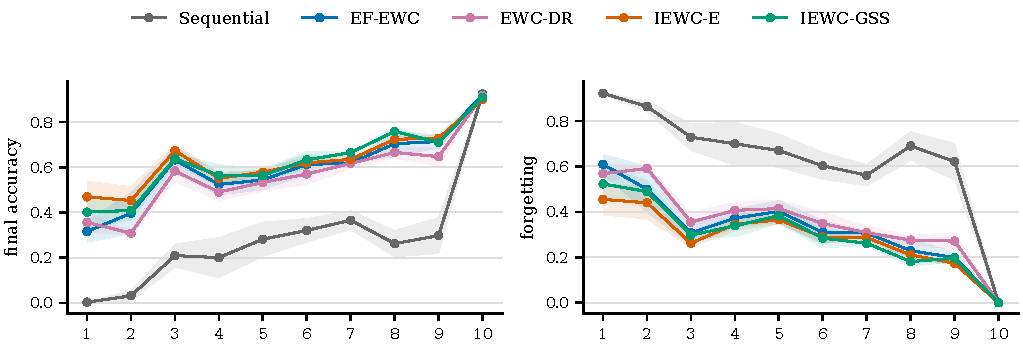
\includegraphics[width=0.65\linewidth]{figures/classification_distribution_retention.pdf}
\caption[ImageNet-R distribution retention]{ImageNet-R distribution retention. The left panel shows the final accuracy on each distribution after the full sequence; the right panel shows the corresponding forgetting. U-IEWC and GSS-IEWC improve retention across most distributions relative to EF-EWC, while sequential training forgets the early distributions almost entirely.}
\label{fig:classification-distribution-retention}
\end{figure}

At the distribution level, Figure \ref{fig:classification-distribution-retention} breaks the classification result down by distribution. The retained accuracy is not concentrated in a single late distribution: the IEWC variants reduce forgetting across the early and middle parts of the sequence, which is the regime where sequential fine-tuning fails most visibly.

\begin{figure}[H]
\centering
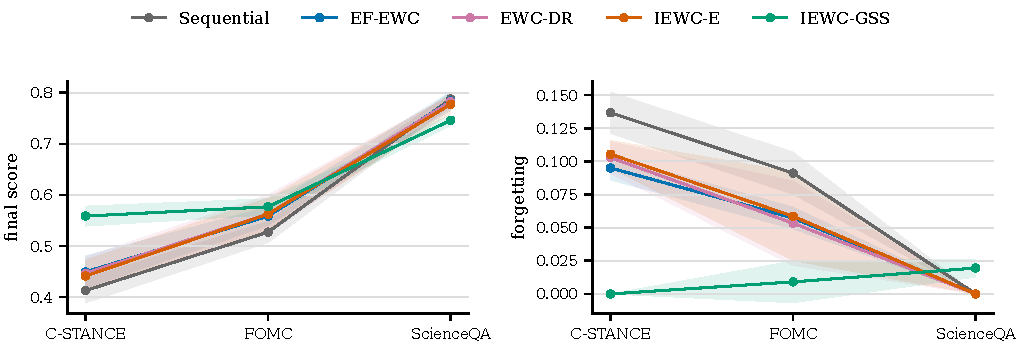
\includegraphics[width=0.65\linewidth]{figures/nlp_distribution_retention.pdf}
\caption[TRACE distribution retention]{TRACE distribution retention. The plot reports the final multiple-choice score and forgetting for C-STANCE, FOMC, and ScienceQA after sequential LoRA fine-tuning of Qwen2.5-3B. GSS-IEWC preserves the earlier NLP distributions while keeping competitive performance on the final distribution.}
\label{fig:nlp-distribution-retention}
\end{figure}

Similarly, the TRACE retention profile in Figure \ref{fig:nlp-distribution-retention} explains the table-level gain of GSS-IEWC. The weighted aggregation mainly changes the stability side of the tradeoff: it reduces forgetting on C-STANCE and FOMC while leaving ScienceQA in the same range as the other regularized methods.

\begin{figure}[H]
\centering
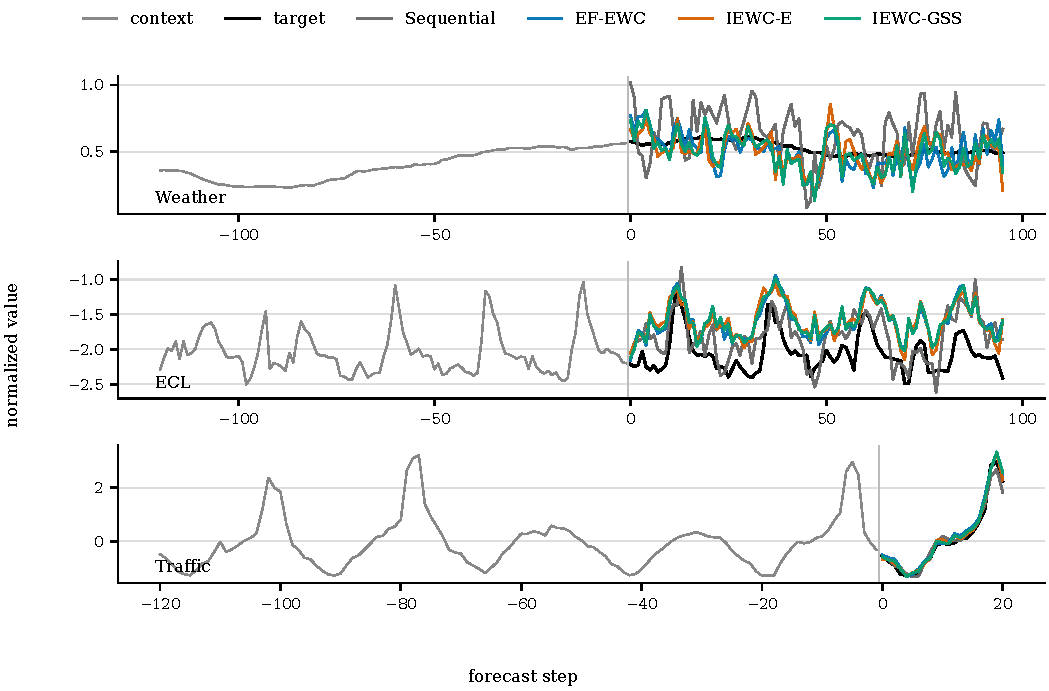
\includegraphics[width=0.75\linewidth]{figures/forecast_rollouts_longhorizon_tasknorm_selected.pdf}
\caption[Forecasting rollout comparison]{Forecasting rollout comparison. Each panel shows one held-out rollout from the corresponding forecasting distribution. The gray curve is the observed context, the black curve is the target horizon, and colored curves are method predictions after the full continual sequence.}
\label{fig:forecast-rollouts}
\end{figure}

For visual inspection and qualitative analysis, Figure \ref{fig:forecast-rollouts} adds individual forecasts. We can see that forgetting significantly affects all methods, while GSS-IEWC retains the most target trajectory structure at the first task and stays close to EF-EWC on later tasks.

In addition, the output-geometry parameter $\Gamma$ is evaluated separately in the DDPM setting. Replacing the Euclidean output metric with a sliced-Wasserstein surrogate lowers old-output sliced-Wasserstein drift relative to Euclidean U-IEWC ($9.4409\pm7.2517$ versus $14.1026\pm12.2220$), while keeping final average denoising MSE close to U-IEWC ($0.0301\pm0.0012$ versus $0.0298\pm0.0014$).

Finally, we tested FROMP-derived sample weighting \citep{FROMP} as a second alternative to the empirical weighting, with mixed results: on ImageNet-R, IEWC-FROMP reaches $0.6365\pm0.0165$ final average accuracy and $0.3068\pm0.0170$ forgetting, slightly ahead of GSS-IEWC; on VOC 15-5, it reaches only $0.3351\pm0.0742$ final all-mIoU and $0.4064\pm0.1122$ base-class forgetting, below U-IEWC and GSS-IEWC.

For reproducibility, Appendix C gives the experimental protocol, the programmatic $\lambda$ search, a damping sensitivity curve, and the effective summand-norm distributions. Appendix D connects the contamination model of Appendix B to a controlled label-noise experiment and reports the resulting accuracy and importance-matrix stability.

\subsection*{Code Release}

We release an accompanying repository with a readily usable IEWC implementation. The \texttt{IEWCConfig} class encapsulates the four-tuple parametrization introduced above. The same configuration interface is used by the diagonal and low-rank IEWC paths and by the empirical scripts, including the FACIL-based CIFAR-100 checks and the larger ImageNet-R, TRACE, forecasting, segmentation, and diffusion runs. The repository is available at \url{https://github.com/Axym-Labs/iewc}.


\section{Limitations}

CLOC is a formulation of preservation, not a claim that all old-task behavior can be retained. Per-sample equality is stronger than expected-risk preservation and can conflict with fitting later tasks. The penalty coefficient therefore controls a stability--plasticity relaxation rather than guaranteeing feasibility of the original hard constraint.

IEWC, like EWC, compresses an old task into one importance matrix evaluated at $\theta_A^\star$ and keeps it fixed during later training. Before aggregation, however, its normalized parameter-sensitivity direction $a^{G}(x;\theta_A^\star)=J_{\theta_A^\star}(x)^\top\hat r^{G}(x)$ is input-dependent. Circuit analyses make the same distinction between a model's fixed connections and the input-dependent feature contributions that realize a particular computation \citep{DunefskyTranscoders}. A single average---especially after diagonalization---can therefore hide sensitivity confined to subsets of inputs or distributed across overlapping pathways, and cannot track changes in the relevant Jacobians as the parameters move away from $\theta_A^\star$. Sample weighting changes which empirical average is stored, but cannot recover this conditional structure after compression. Conditional mixtures or dynamically refreshed importance are natural extensions, at the cost of richer stored summaries or access to old inputs.

The output metric must be specified as a matched primal/dual pair. Ambient singular metrics require restriction to an identifiable subspace and a stated pseudoinverse convention. Our ordered-CDF construction satisfies that requirement on the probability-simplex tangent, but the inherited diffusion result is exploratory and does not validate a general Wasserstein geometry.

Practical IEWC also introduces approximations beyond the derivation. A diagonal retains coordinatewise importance but discards correlations, eigenspaces, and reparameterization behavior. Importance estimates use finitely many old samples. RDW is an order-dependent weighting heuristic with additional cost and is not implied by level-set normalization. Relative damping guarantees invariance to a global change of loss units, not to arbitrary sample-dependent transformations at finite damping.

Finally, empirical comparisons cover selected datasets, model families, adaptation regimes, and task orders. Validation selection and locked paired evaluation reduce selection bias but cannot establish a domain-independent advantage or deployment robustness. Offline/joint training is only a reference because it violates the continual data-access constraint, and untested replay, distillation, and parameter-isolation methods may be preferable when their storage or architectural assumptions are allowed.


\section{Conclusion}

We formulated continual learning as an old-solution preservation constraint (CLOC) and derived two local quadratic relaxations. Preserving each old sample's scalar loss yields an outer-product loss-gradient matrix; for negative log likelihood, this is algebraically the observed-label empirical Fisher used in many EWC implementations, but it is not the model Fisher or a general curvature identity. Preserving outputs modulo the tangent to the old loss level set instead yields the iEF normalization. This retains the central geometric intuition while locating its exact boundary: undamped normalization removes the samplewise output-loss-gradient scale, whereas positive damping multiplies each summand by $s/(s+\tau)$ and assigns zero contribution at exact interpolation.

Task-relative damping restores invariance to global changes of loss units, and the controlled contamination study directly shows that normalization can prevent high-loss corrupted samples from dominating a full importance matrix in the tested construction. Whether this altered local geometry improves a diagonal continual-learning penalty remains an empirical, domain-conditional question. Our evaluation therefore separates normalization from residual-diversity weighting, matches global scale, includes external regularization and offline references, selects hyperparameters only on validation data, and reserves paired task orders and test splits for locked inference. IEWC is best understood as a CLOC-derived family whose damping, weighting, output metric, and matrix approximation are explicit choices---not as a universal replacement for every continual-learning method.


\bibliographystyle{unsrtnat}
\bibliography{references}

\appendix

\section{Invariance to Loss Reparameterization}

This appendix treats the undamped case $\tau=0$.

The output-level feasible set

\[
\mathcal C_n=\{z:\ell_n(z)=\ell_n(z_n^A)\}
\]

depends on the level sets of $\ell_n$, not on the numerical labels assigned to those level sets. If we apply a local monotone scalar transformation

\[
\tilde \ell=\phi(\ell),
\qquad
\phi'(\ell)>0,
\]

then the output gradient rescales as

\[
\tilde r_n
=
\phi'(\ell_n(z_n^A))\,r_n.
\]

For OPG, the sample contribution changes by

\[
J_n^\top \tilde r_n\tilde r_n^\top J_n
=
\phi'(\ell_n(z_n^A))^2
J_n^\top r_nr_n^\top J_n.
\]

For IEF, the same scalar factor appears in numerator and denominator:

\[
\frac{\tilde r_n\tilde r_n^\top}
{\tilde r_n^\top G_n^{-1}\tilde r_n}
=
\frac{r_nr_n^\top}
{r_n^\top G_n^{-1}r_n}.
\]

Thus undamped IEF is invariant to local scalar relabelings of the constraint function wherever $r_n\ne0$. This includes loss rescaling, unit changes in regression losses, reduction conventions, and smooth monotone transformations that preserve the local level-set geometry. OPG's global scale can be absorbed into $\lambda$ only when the transformation rescales all samples equally; sample-dependent factors change its relative weighting.

Positive shared damping narrows the invariance. A fixed numerical $\tau$ does not transform with the loss and therefore changes even under a global unit rescaling. Task-relative damping $\tau_A=\kappa\operatorname{median}_{i:s_i>0}s_i$ restores invariance to a global task-loss multiplier because $s_i$ and $\tau_A$ scale together. It does not generally preserve invariance to sample-dependent monotone transformations. At $r_n=0$, the implementation assigns a zero contribution rather than claiming an undamped $0/0$ identity.


\section{Spectral Stability Under Contamination}

The normalization difference between EF and IEF has consequences for their spectrum. This matters in practice because any diagonal or low-rank approximation is built from the leading part of the matrix. Consider for example \citep{Rank1Diffusion}. To see how this difference can affect the leading eigenspace, consider the following simple contamination model: Contaminated samples, such as mislabeled or atypical data, can have large output-loss gradients because their signal aligns with directions that gradient descent learns only very slowly; in the spectral-bias / kernel-eigenmode framework, low-alignment or low-eigenvalue components can remain effectively unlearned over the training horizon \citep{Memorization,SpectralBias}. With probability $1-\varepsilon$, a sample is clean and its normalized sensitivity direction contributes to a stable old-task preservation matrix $\Sigma_{\mathrm{clean}}=\mathbb E[a a^\top \mid a \in D_{A,\mathrm{clean}}]$. Assume also that clean weights are independent of these normalized directions, or are sufficiently concentrated around their clean mean. With probability $\varepsilon$, a sample is contaminated. Assume its direction is concentrated near a unit vector $u$ outside that clean leading subspace, and that its output gradient scale is large,
\[
w \approx W,  
\qquad  
W\gg 1.
\]
Under this model, the population version of IEF is
\[
\mathbb E[M_{\mathrm{IEF}}]
= (1-\varepsilon)\Sigma_{\mathrm{clean}}
+  
\varepsilon uu^\top
\]
while the corresponding EF matrix becomes
\[
\mathbb E[F_{\mathrm{EF}}]
=
(1-\varepsilon)\mathbb E[w\mid\text{clean}]\,\Sigma_{\mathrm{clean}}  
+  
\varepsilon W uu^\top.  
\]

In terms of the spectrum, let $\lambda_k^{\mathrm{clean}}$ denote the $k$-th eigenvalue of the clean component. If
\[
\varepsilon W  
\gtrsim  
(1-\varepsilon)\lambda_k^{\mathrm{clean}}\mathbb E[w\mid\text{clean}],  
\]
then the contaminated direction $u$ will enter the leading eigenspace of $F_{\mathrm{EF}}$. The insight is that the normalization can realistically affect which directions dominate the spectrum. In settings with noisy labels, hard examples, underfit outliers, or other rare but high-loss samples, we should expect the leading eigenspace of $F_{\mathrm{EF}}$ to be less stable than that of $M_{\mathrm{IEF}}$, relevant to low-rank approximations thereof.


\section{Experimental Details and Damping Sensitivity}

\textbf{Training and Tuning Protocol} Table \ref{tab:empirical-protocol} summarizes the paper-facing empirical runs. The tuning objective is the final average performance across all distributions in a sequence. For MSE-based tasks this means lower final average MSE; for accuracy, score, and mIoU it means higher final average performance. Forgetting is then reported as a separate retention metric rather than used as the primary tuning objective.

\begin{table}[H]
\centering
\small
\resizebox{\linewidth}{!}{%
\begin{tabular}{@{}p{0.10\linewidth}p{0.17\linewidth}p{0.12\linewidth}p{0.075\linewidth}p{0.10\linewidth}p{0.38\linewidth}@{}}
\toprule
Task type & Dataset and sequence & Model & Pretrained & Training regime & Selected regularization values \\
\midrule
Classification & ImageNet-R, ten 20-class distributions & ViT-B/16 & Yes & LoRA, rank 4 & \begin{tabular}[t]{@{}l@{}}EF: $\lambda=333.333$\\DR: $\lambda=3$\\U-IEWC: $\lambda=33.333,\tau=10^{-4}$\\GSS-IEWC: $\lambda=11.111,\tau=10^{-2}$\end{tabular} \\
NLP & TRACE: C-STANCE $\rightarrow$ FOMC $\rightarrow$ ScienceQA & Qwen2.5-3B & Yes & LoRA, rank 8 & \begin{tabular}[t]{@{}l@{}}EF: $\lambda=1$\\DR: $\lambda=1$\\U-IEWC: $\lambda=0.111,\tau=10^{-2}$\\GSS-IEWC: $\lambda=59049,\tau=10^{-2}$\end{tabular} \\
Forecasting & Weather $\rightarrow$ ECL $\rightarrow$ Traffic & PatchTST & No & From scratch & \begin{tabular}[t]{@{}l@{}}EF: $\lambda=729$\\U-IEWC: $\lambda=9,\tau=10^{-2}$\\GSS-IEWC: $\lambda=9,\tau=10^{-2}$\end{tabular} \\
Segmentation & VOC 15-5, base classes then novel classes & ConvNeXtV2-tiny FPN & Yes & Full fine-tuning & \begin{tabular}[t]{@{}l@{}}EF: $\lambda=0.111$\\DR: $\lambda=243$\\U-IEWC: $\lambda=270,\tau=10^{-3}$\\GSS-IEWC: $\lambda=2430,\tau=10^{-2}$\end{tabular} \\
Diffusion & MNIST DDPM, labels $0/1\rightarrow2/3$ & Conditional DDPM & No & From scratch & \begin{tabular}[t]{@{}l@{}}EF: $\lambda=9\cdot10^5$\\U-IEWC: $\lambda=675,\tau=10^{-3}$\\GSS-IEWC: $\lambda=225,\tau=10^{-3}$\\IEWC-SW: $\lambda=10^6,\tau=10^{-3}$\end{tabular} \\
\bottomrule
\end{tabular}
}
\caption[Empirical training and tuning protocol]{Empirical training and tuning protocol for the main paper-facing runs. ``DR'' denotes EWC-DR. IEWC-SW is the sliced-Wasserstein output-geometry ablation discussed outside the main table.}
\label{tab:empirical-protocol}
\end{table}

The $\lambda$ search is programmatic. For each regularized method, we evaluate a five-point multiplicative grid centered at a task-specific midpoint. The midpoint is either the selected value from a validated predecessor in the same task family or the best value from a short seed-0 scale probe. If the best point lies on a grid boundary, we extend the grid in that direction, with at most three such extensions. The selected $\lambda$ is then rerun on the remaining seeds. This keeps the tuning objective fixed while avoiding ad hoc one-off extensions.

\textbf{Damping Sensitivity on CIFAR-100} Figure \ref{fig:tau-sensitivity-cifar100} reports a separate damping sensitivity experiment on CIFAR-100 with FACIL, the iCaRL class order, ResNet-32, and the first three distributions of the ten-distribution task-aware protocol. Each distribution is trained for 60 epochs. IEWC uses a diagonal matrix surrogate, 512 old-distribution samples for the importance estimate, and importances scale-matched to the corresponding EF estimate so that the EF regularization strength can be reused.

\begin{figure}[H]
\centering
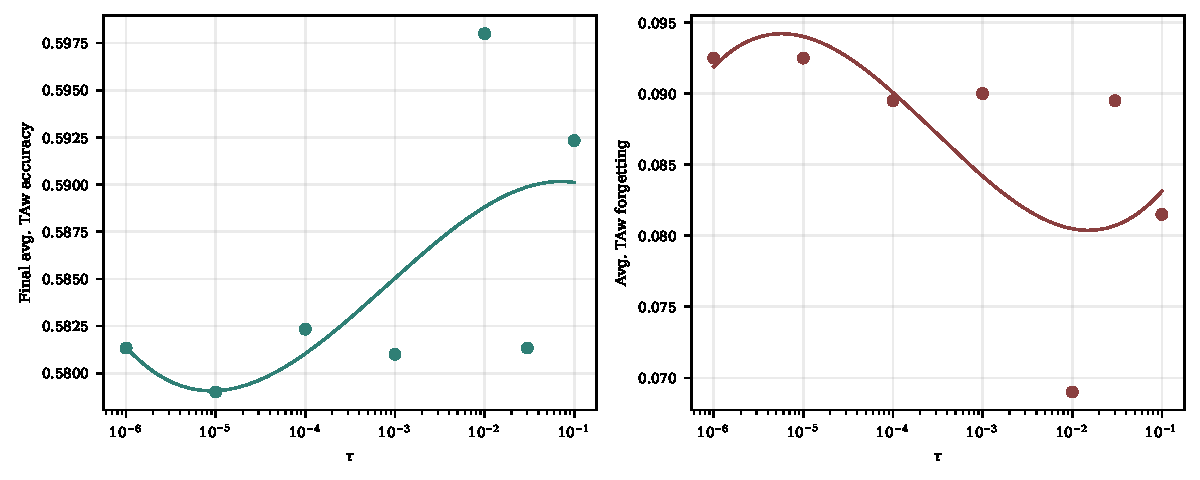
\includegraphics[width=0.62\linewidth]{figures/tau_sensitivity_cifar100.pdf}
\caption[Tau sensitivity on CIFAR-100]{Tau sensitivity on CIFAR-100. The tested values are $\{10^{-6},10^{-5},10^{-4},10^{-3},10^{-2},3\cdot10^{-2},10^{-1}\}$. The damping parameter has a measurable effect on this ResNet/FACIL prefix protocol: $\tau=10^{-2}$ gives the highest final task-aware accuracy and lowest forgetting among the tested values, so we use it as a practical default before task-specific tuning.}
\label{fig:tau-sensitivity-cifar100}
\end{figure}

\textbf{Effective Summand Norms} Figure \ref{fig:summand-norm-ecdf} reports a separate scale diagnostic from the original diagonal-analysis suite: CIFAR-100 classification, controlled regression, MNIST DDPM denoising, and the earlier binary segmentation setup. The plot shows the effective scale of the diagonal summands after multiplication by the corresponding $\lambda$. It is not a sample-weight plot, because the unweighted U-IEWC mechanism uses $h_n\equiv 1$.

\begin{figure}[H]
\centering
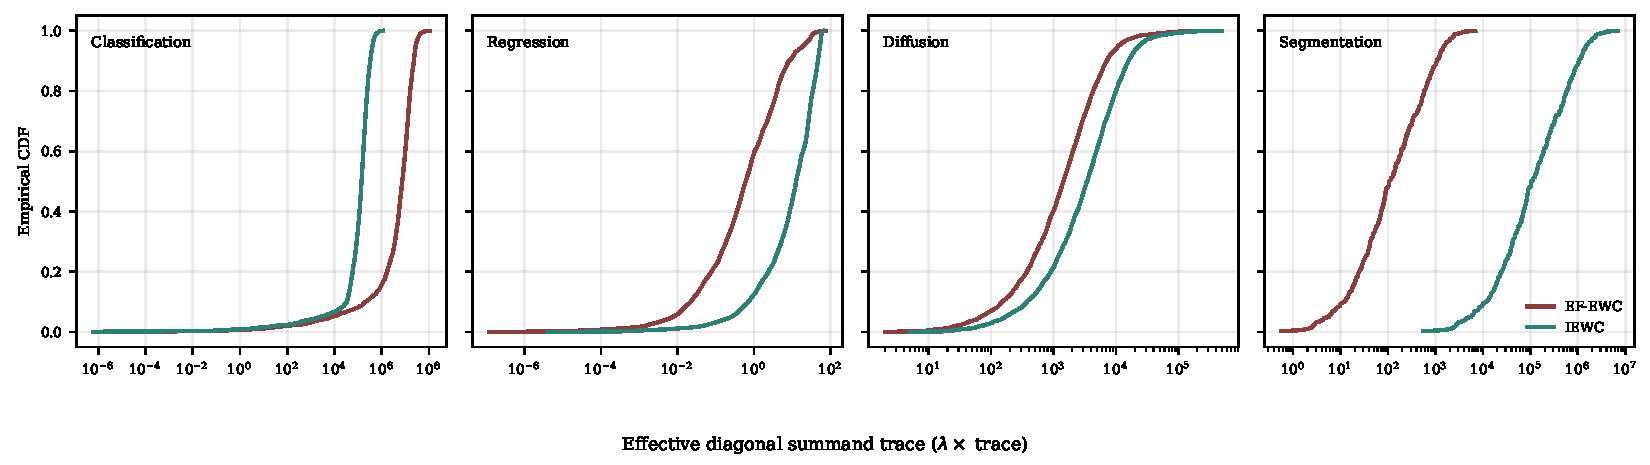
\includegraphics[width=0.95\linewidth]{figures/summand_norm_ecdf.pdf}
\caption[Effective diagonal summand norms]{Effective diagonal summand norms. Each panel reports the empirical CDF of $\lambda$ times the per-sample diagonal summand trace before averaging over old-distribution samples, with EF-EWC and IEWC shown on the same diagnostic task type.}
\label{fig:summand-norm-ecdf}
\end{figure}

For EWC-DR, we additionally checked $\lambda\in\{100,300,1000,3000,10000\}$ on the CIFAR-100 three-distribution prefix used for the damping plot. The best tested value on this prefix was $\lambda=100$; we use this only as a local parameter-sensitivity check for the earlier CIFAR-100 setup, not as the tuning protocol for the ImageNet-R results in Table \ref{tab:main-empirical-results}.


\section{Label-Noise Stress Test}

The contamination model in Appendix B predicts that rare high-loss samples can dominate EF-EWC because their loss-gradient scales enter the empirical Fisher directly. Controlled label noise instantiates this mechanism: corrupted labels create atypical high-loss training samples, while clean task-aware test sets measure whether the stored preservation matrix still protects the original classification structure. We therefore add uniform label noise to the CIFAR-100 training data in FACIL and report final average task-aware accuracy. IEWC degrades much more slowly than EF-EWC as the label-noise rate increases.

\begin{table}[t]
\centering
\begin{tabular}{lrrr}
\toprule
Method & $p=0$ & $p=0.1$ & $p=0.25$ \\
\midrule
EF-EWC & 0.5617 $\pm$ 0.0062 & 0.5132 $\pm$ 0.0112 & 0.2773 $\pm$ 0.0320 \\
EWC-DR & 0.5932 $\pm$ 0.0296 & 0.5310 $\pm$ 0.0226 & 0.4598 $\pm$ 0.0095 \\
IEWC & 0.5978 $\pm$ 0.0260 & 0.5642 $\pm$ 0.0215 & 0.5322 $\pm$ 0.0239 \\
\bottomrule
\end{tabular}
\end{table}

To connect this performance effect to the matrix-level prediction of the contamination model, we also record the largest stored diagonal entries of the EF and IEWC matrices on the same CIFAR-100 prefix protocol. These are not low-rank approximations. For diagonal matrices, the relevant stability object is the high-importance coordinate tail, so the table uses all 512 exported entries per matrix and reports the stored-tail mass ratio, the normalized stored-tail profile change, and the log-scale RMSE of the sorted entries. EF-EWC changes much more under contamination than IEWC on the log-scale metric.

\begin{table}[t]
\centering
\begin{tabular}{lrrrrr}
\toprule
Method & Noise & Entries & Stored-tail mass ratio & Stored-tail profile L1 & Stored-tail log-scale RMSE \\
\midrule
EF-EWC & 0.1 & 512 & 0.0288 & 0.2610 & 1.4660 \\
EF-EWC & 0.25 & 512 & 0.0244 & 0.2737 & 1.5337 \\
IEWC & 0.1 & 512 & 1.0833 & 0.0350 & 0.0350 \\
IEWC & 0.25 & 512 & 1.1003 & 0.0154 & 0.0415 \\
\bottomrule
\end{tabular}
\end{table}

\begin{figure}[H]
\centering
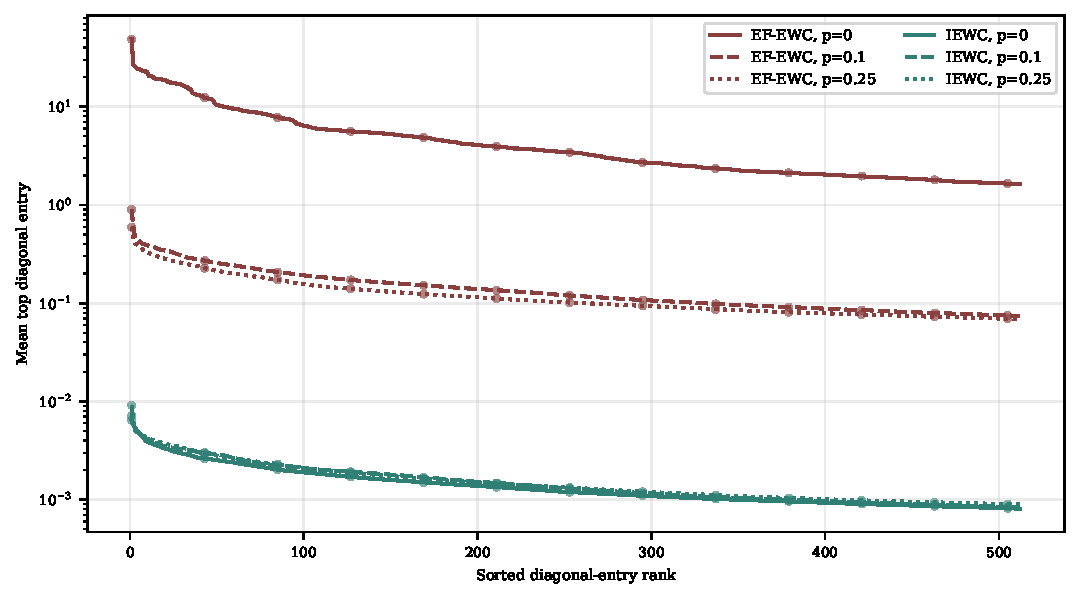
\includegraphics[width=0.54\linewidth]{figures/contamination_diagonal_spectra.pdf}
\caption[Label-noise diagonal spectra]{Label-noise diagonal spectra. The plot visualizes the high-importance coordinate tail underlying the matrix-level comparison above; EF-EWC changes much more under contamination than IEWC on the log scale.}
\label{fig:contamination-diagonal-spectra}
\end{figure}

\end{document}
